\documentclass[tikz,border=2pt,11pt]{standalone}
\usetikzlibrary{arrows.meta}
\usetikzlibrary{calc}
\usetikzlibrary{positioning}
\usepackage{amsmath}
\usepackage{amssymb}
\usepackage{mathrsfs}
\usepackage{bm}
\usepackage{tikz}
\newcommand{\R}{\mathbb R}
\newcommand{\N}{\mathbb N}
\newcommand{\Z}{\mathbb Z}
\newcommand{\dd}{\,\mathrm d}
\DeclareMathOperator{\tr}{tr}
\DeclareMathOperator{\Div}{div}
\DeclareMathOperator{\divg}{div}
\DeclareMathOperator{\Ric}{Ric}
\DeclareMathOperator{\Hess}{Hess}
\DeclareMathOperator{\supp}{supp}
\DeclareMathOperator{\sym}{sym}
\DeclareMathOperator{\Sym}{Sym}
\DeclareMathOperator{\Vol}{Vol}
\DeclareMathOperator{\Scal}{Scal}
\DeclareMathOperator{\scal}{Scal}
\DeclareMathOperator{\grad}{grad}
\DeclareMathOperator{\Id}{Id}
\DeclareMathOperator{\id}{id}
\DeclareMathOperator{\rank}{rank}
\DeclareMathOperator{\Lip}{Lip}
\DeclareMathOperator{\sgn}{sgn}
\DeclareMathOperator{\Area}{Area}
\DeclareMathOperator{\dist}{dist}
\newcommand{\Mext}{M_{\mathrm{ext}}}
\newcommand{\Achi}{A_\chi}
\newcommand{\Ad}{A_d}
\newcommand{\cT}{\mathcal T}
\newcommand{\gbar}{\bar g}
\newcommand{\ghat}{\widehat g}
\newcommand{\cB}{\mathcal B}
\newcommand{\cE}{\mathcal E}
\newcommand{\cP}{\mathcal P}
\newcommand{\cD}{\mathcal D}
\newcommand{\cW}{\mathcal W}
\newcommand{\eps}{\epsilon}
\newcommand{\omegaThree}{\omega_3}
\newcommand{\abs}[1]{\lvert#1\rvert}
\newcommand{\norm}[1]{\lVert#1\rVert}
\newcommand{\inner}[2]{\langle#1,#2\rangle}
\newcommand{\AH}{\mathrm{AH}}
\newcommand{\II}{\mathrm{II}}
\newcommand{\tf}{\circ}
\begin{document}
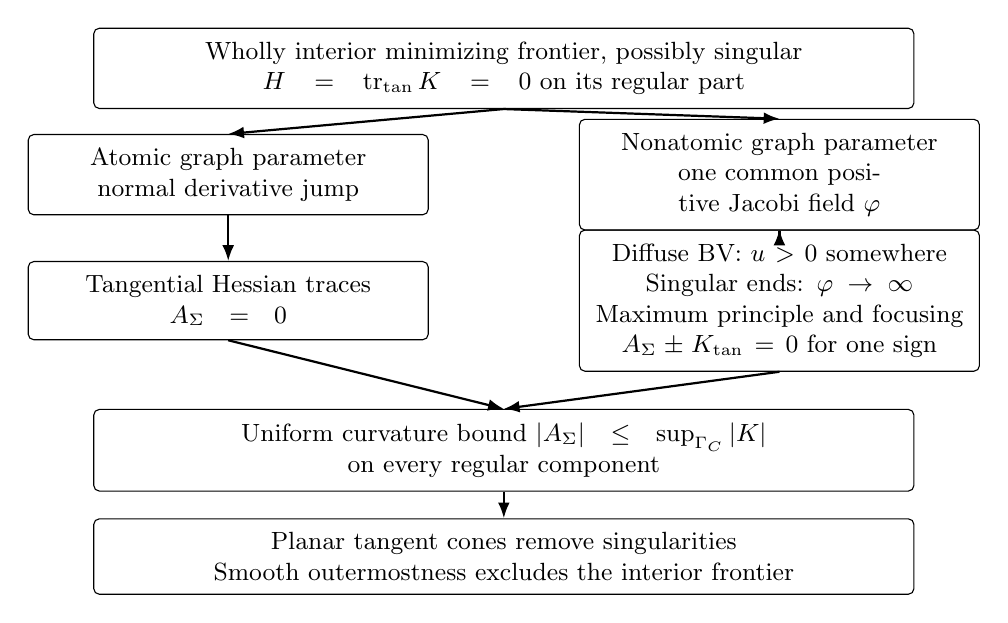
\begin{tikzpicture}[
 box/.style={draw,rounded corners=2pt,align=center,font=\small,
             inner sep=5pt,text width=.39\linewidth},
 flow/.style={-{Latex[length=2mm]},thick}]
 \node[box,text width=.83\linewidth] (family) at (0,0)
   {Wholly interior minimizing frontier, possibly singular\\
    $H=\tr_{\rm tan}K=0$ on its regular part};
 \node[box] (atom) at (-3.5,-1.35)
   {Atomic graph parameter\\
    normal derivative jump};
 \node[box] (nonatomic) at (3.5,-1.35)
   {Nonatomic graph parameter\\
    one common positive Jacobi field $\varphi$};
 \node[box] (flat) at (-3.5,-2.95)
   {Tangential Hessian traces\\
    $A_\Sigma=0$};
 \node[box] (maximum) at (3.5,-2.95)
   {Diffuse BV: $u>0$ somewhere\\
    Singular ends: $\varphi\to\infty$\\
    Maximum principle and focusing\\
    $A_\Sigma\pm K_{\rm tan}=0$ for one sign};
 \node[box,text width=.83\linewidth] (bound) at (0,-4.85)
   {Uniform curvature bound $|A_\Sigma|\le\sup_{\Gamma_C}|K|$\\
    on every regular component};
 \node[box,text width=.83\linewidth] (finish) at (0,-6.2)
   {Planar tangent cones remove singularities\\
    Smooth outermostness excludes the interior frontier};
 \draw[flow] (family.south) -- (atom.north);
 \draw[flow] (family.south) -- (nonatomic.north);
 \draw[flow] (atom) -- (flat);
 \draw[flow] (nonatomic) -- (maximum);
 \draw[flow] (flat.south) -- (bound.north);
 \draw[flow] (maximum.south) -- (bound.north);
 \draw[flow] (bound) -- (finish);
\end{tikzpicture}
\end{document}
